% This file was created with tikzplotlib v0.10.1.
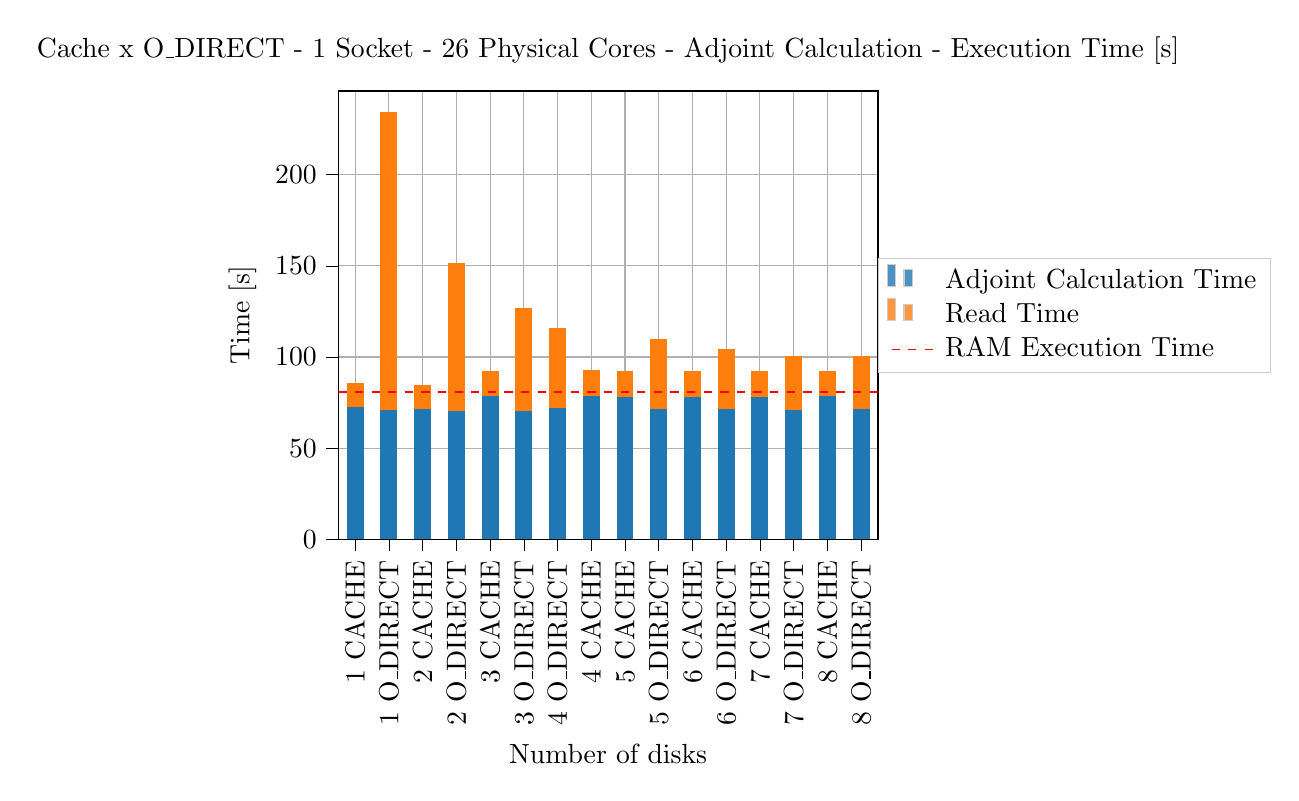
\begin{tikzpicture}

\definecolor{darkgray176}{RGB}{176,176,176}
\definecolor{darkorange25512714}{RGB}{255,127,14}
\definecolor{lightgray204}{RGB}{204,204,204}
\definecolor{steelblue31119180}{RGB}{31,119,180}

\begin{axis}[
legend cell align={left},
legend style={
  fill opacity=0.8,
  draw opacity=1,
  text opacity=1,
  at={(1,0.5)},
  anchor=west,
  draw=lightgray204
},
tick align=outside,
tick pos=left,
title={Cache x O\_DIRECT - 1 Socket - 26 Physical Cores - Adjoint Calculation - Execution Time [s]},
x grid style={darkgray176},
xlabel={Number of disks},
xmajorgrids,
xmin=-0.5, xmax=15.5,
xtick style={color=black},
xtick={0,1,2,3,4,5,6,7,8,9,10,11,12,13,14,15},
xticklabel style={rotate=90.0},
xticklabels={
  1 CACHE,
  1 O\_DIRECT,
  2 CACHE,
  2 O\_DIRECT,
  3 CACHE,
  3 O\_DIRECT,
  4 O\_DIRECT,
  4 CACHE,
  5 CACHE,
  5 O\_DIRECT,
  6 CACHE,
  6 O\_DIRECT,
  7 CACHE,
  7 O\_DIRECT,
  8 CACHE,
  8 O\_DIRECT
},
y grid style={darkgray176},
ylabel={Time [s]},
ymajorgrids,
ymin=0, ymax=245.91,
ytick style={color=black}
]
\draw[draw=none,fill=steelblue31119180] (axis cs:-0.25,0) rectangle (axis cs:0.25,72.46);
\addlegendimage{ybar,ybar legend,draw=none,fill=steelblue31119180}
\addlegendentry{Adjoint Calculation Time}

\draw[draw=none,fill=steelblue31119180] (axis cs:0.75,0) rectangle (axis cs:1.25,71.07);
\draw[draw=none,fill=steelblue31119180] (axis cs:1.75,0) rectangle (axis cs:2.25,71.48);
\draw[draw=none,fill=steelblue31119180] (axis cs:2.75,0) rectangle (axis cs:3.25,70.46);
\draw[draw=none,fill=steelblue31119180] (axis cs:3.75,0) rectangle (axis cs:4.25,78.78);
\draw[draw=none,fill=steelblue31119180] (axis cs:4.75,0) rectangle (axis cs:5.25,70.52);
\draw[draw=none,fill=steelblue31119180] (axis cs:5.75,0) rectangle (axis cs:6.25,71.73);
\draw[draw=none,fill=steelblue31119180] (axis cs:6.75,0) rectangle (axis cs:7.25,78.55);
\draw[draw=none,fill=steelblue31119180] (axis cs:7.75,0) rectangle (axis cs:8.25,78.29);
\draw[draw=none,fill=steelblue31119180] (axis cs:8.75,0) rectangle (axis cs:9.25,71.47);
\draw[draw=none,fill=steelblue31119180] (axis cs:9.75,0) rectangle (axis cs:10.25,78.12);
\draw[draw=none,fill=steelblue31119180] (axis cs:10.75,0) rectangle (axis cs:11.25,71.21);
\draw[draw=none,fill=steelblue31119180] (axis cs:11.75,0) rectangle (axis cs:12.25,78.13);
\draw[draw=none,fill=steelblue31119180] (axis cs:12.75,0) rectangle (axis cs:13.25,71.16);
\draw[draw=none,fill=steelblue31119180] (axis cs:13.75,0) rectangle (axis cs:14.25,78.37);
\draw[draw=none,fill=steelblue31119180] (axis cs:14.75,0) rectangle (axis cs:15.25,71.45);
\draw[draw=none,fill=darkorange25512714] (axis cs:-0.25,72.46) rectangle (axis cs:0.25,85.47);
\addlegendimage{ybar,ybar legend,draw=none,fill=darkorange25512714}
\addlegendentry{Read Time}

\draw[draw=none,fill=darkorange25512714] (axis cs:0.75,71.07) rectangle (axis cs:1.25,234.2);
\draw[draw=none,fill=darkorange25512714] (axis cs:1.75,71.48) rectangle (axis cs:2.25,84.36);
\draw[draw=none,fill=darkorange25512714] (axis cs:2.75,70.46) rectangle (axis cs:3.25,151.41);
\draw[draw=none,fill=darkorange25512714] (axis cs:3.75,78.78) rectangle (axis cs:4.25,92.3);
\draw[draw=none,fill=darkorange25512714] (axis cs:4.75,70.52) rectangle (axis cs:5.25,126.92);
\draw[draw=none,fill=darkorange25512714] (axis cs:5.75,71.73) rectangle (axis cs:6.25,115.79);
\draw[draw=none,fill=darkorange25512714] (axis cs:6.75,78.55) rectangle (axis cs:7.25,92.59);
\draw[draw=none,fill=darkorange25512714] (axis cs:7.75,78.29) rectangle (axis cs:8.25,92.27);
\draw[draw=none,fill=darkorange25512714] (axis cs:8.75,71.47) rectangle (axis cs:9.25,109.63);
\draw[draw=none,fill=darkorange25512714] (axis cs:9.75,78.12) rectangle (axis cs:10.25,92.09);
\draw[draw=none,fill=darkorange25512714] (axis cs:10.75,71.21) rectangle (axis cs:11.25,104.5);
\draw[draw=none,fill=darkorange25512714] (axis cs:11.75,78.13) rectangle (axis cs:12.25,92.09);
\draw[draw=none,fill=darkorange25512714] (axis cs:12.75,71.16) rectangle (axis cs:13.25,100.51);
\draw[draw=none,fill=darkorange25512714] (axis cs:13.75,78.37) rectangle (axis cs:14.25,92.35);
\draw[draw=none,fill=darkorange25512714] (axis cs:14.75,71.45) rectangle (axis cs:15.25,100.54);
\addplot [semithick, red, dashed]
table {%
-0.5 80.83
15.5 80.83
};
\addlegendentry{RAM Execution Time}
\end{axis}

\end{tikzpicture}
